\chapter{The CMS Tracker Upgrade}\label{chapter:tk-upgrade}
 
\section{The High-Luminosity Large Hadron Collider} \label{sec:hl-lhc}
The High-Luminosity Large Hadron Collider (HL-HLC) upgrade is expected to be installed during Long Shutdown 3 (2023-2025), with the instantaneous luminosity of the LHC increasing up to $5-7.5 \times {10}^{34}$\percms, corresponding to an average number of proton-proton interactions per 40\MHz bunch crossing of 140 to 200, and a total integrated luminosity of 3000\fbinv to the ATLAS and CMS experiments.

Increasing the LHC's instantaneous luminosity is motivated by the need to replace the inner triplet quadrupole magnets which focus the beams at the ATLAS and CMS collision regions, that are expected to be near life expired due to radiation exposure by 2023~\cite{hl-lhc-prelim-design-report,CMSCollaboration:2015zni}.
This increase in instantaneous luminosity will provide the experiments the ability to overcome the diminishing statistical gains that occur the longer an experiment is operated for at constant luminosity, and so enable greater precision SM and Higgs measurements, searches for rare processes and their potential deviations from the SM, and the discovery reach for multi-\TeV massive particles.

The instantaneous luminosity of the machine and the beam parameters are related by: the number of bunches $n_{b}$, the number of protons per bunch $N^{2}_{p}$, the beam beta value (focal length) at the collision point $\beta^{*}$, and a crossing angle dependent luminosity geometrical reduction factor $R$,

\begin{equation}
L \propto \frac{n_{b}N^{2}_{p}}{\beta^{*}} R \\
\label{eq:machineLumi}
\end{equation}

As it is not practical to increase the number of proton bunches due to the resultant heat loads induced by electron clouds, the increase in the machine's luminosity will be achieved by increasing the number of protons per bunch and by  reducing $\beta^{*}$.
Replacing Linac2 with the new Linear accelerator 4 (Linac4) during the Long Shutdown 2 (2019-2020) will allow for the number of protons per bunch to be increased by a factor of two compared to the nominal LHC design (and to increase the injection energy by a factor of three)~\cite{linac4}.
The new more radiation tolerant quadrupole magnets to be installed during LS3 will provide the larger magnetic field strength and aperture required to provide the lower $\beta^{*}$ required for increasing the instantaneous luminosity. 

\section{The Phase-II Outer Tracker Upgrade}\label{sec:tk-upgrade}

To meet the significant challenges of, and exploit, the increased instantaneous luminosity environment of the HL-LHC, the CMS detector's ``Phase-II Upgrade'' during the LS3 will deliver the required improved radiation hardness for the increase in radiation and to manage the high \PU HL-LHC environment with greater detector granularity to reduce occupancy, and enhanced bandwidth and triggering capabilities to avoid compromising physics potential~\cite{CMSCollaboration:2015zni,P2TrackerTDR}.

The Phase-II upgrade will see both the entire silicon tracking detector being replaced with one comprised of a pixel Inner Tracker and pixel and strip Outer Tracker which have:
\begin{itemize}
\item \bf{improved radiation hardness} - being able to withstand the increased fluence of the HL-LHC (up to $2.3\times10^{16} n_{eq}/cm^{2}$ for the innermost layers)and operate efficiently up to the targeted luminosity of 3000\fbinv, with a margin of $\approx50\%$ to accommodate the target being exceeded and the uncertainties in the anticipated radiation exposure.
\item \bf{increased sensor granularity} - so that the channel occupancy is kept at or below the per cent (per mille) level for the Outer (Inner) Tracker, allowing for a high track reconstruction efficiency and a low misidentification rate under the increased \PU conditions. This will also enable improved track separation in dense environments, such as high \pT jets, compared to the current pixel detector and fully exploit the vast volume of data produced.
\item \bf{reduced material in the tracking volume} - the current tracker's performance is significantly impacted by the amount of material present, as are the calorimeters and overall performance of CMS.
Significant reducing the tracker's material budget will greatly enhance CMS' performance at the HL-LHC.
\item \bf{robust pattern recognition} - enabling fast and efficient track finding, which is especially important for the HLT, in the high \PU environment.
\item \bf{level-1 trigger contributions} - it has been shown that the L1 trigger performance will deteriorate in the high luminosity environment from both the rate increase and the reduced efficiencies of the L1 selection algorithms.
As raising the upgraded calorimeters' and muon chambers' trigger thresholds would have minimal impact on the rate, and 	would negatively impact sensitivity to low mass searches and measurements, the L1 bandwidth and latency will be increased and tracking information will be included in the L1 decision process to preserve and improve trigger performance.
\item \bf{extended tracking acceptance} - the overall physics capabilities of the CMS experiment would greatly benefit from extended coverage of the tracker and calorimeters up to $|\eta| = 4$ in the forward region.
\end{itemize}

With the above requirements in mind, the pixel Inner Tracker is designed to cover up to $|\eta| = 4$ with $100-150\mum$ thick planar silicon pixel sensors, measuring either $25\times100\mum^{2}$ or $50\times50\mum^{2}$\footnote{This is a reduction of a factor of $\approx 6$ compared to the Phase-0 and Phase-I pixel detectors}, which provide the low (per mille) occupancy and track separation with the negligible inefficiencies required in the harsh radiation environment.
Akin to the previous pixel detectors, the Phase-II pixel is also designed for easy installation and removal to facilitate the replacement of degraded parts.
Further discussion of the Inner Tracker is detailed in the Phase-II Technical Design Report~\cite{P2TrackerTDR}.

As tracking information is required to make L1 decisions at the HL-LHC, the design of the Outer Tracker has been driven by the need to provide tracking information to the L1 trigger.
Whilst the the L1 bandwidth and latency will be increased to from 100\kHz to 750\kHz and from $3.2\mus$ to $12.5\mus$ respectively, given the bandwidth implications for reading out every hit for the L1 trigger, a novel design of a pair of closely spaced silicon sensors, capable of rejecting hits generated by low \pT particles, has been proposed~\cite{jjonespixel,markthesis}.
The proposed ``\pT module''~\cite{jjonespixel,markthesis} discriminates on charged particle \pT based on the local bend of the track within the magnetic field, as shown in Fig.~\ref{fig:stubs}.
Pairs of clusters which are consistent with a track \pT above a configurable threshold (typically 2-3\GeV) are correlated on-detector, and the resultant \emph{stubs} are transferred to the L1 trigger, providing an effective data rate reduction of approximately a factor of 10~\cite{mpessimperf,2dptmoduleconcept}.

\begin{figure}[!t]
\centering
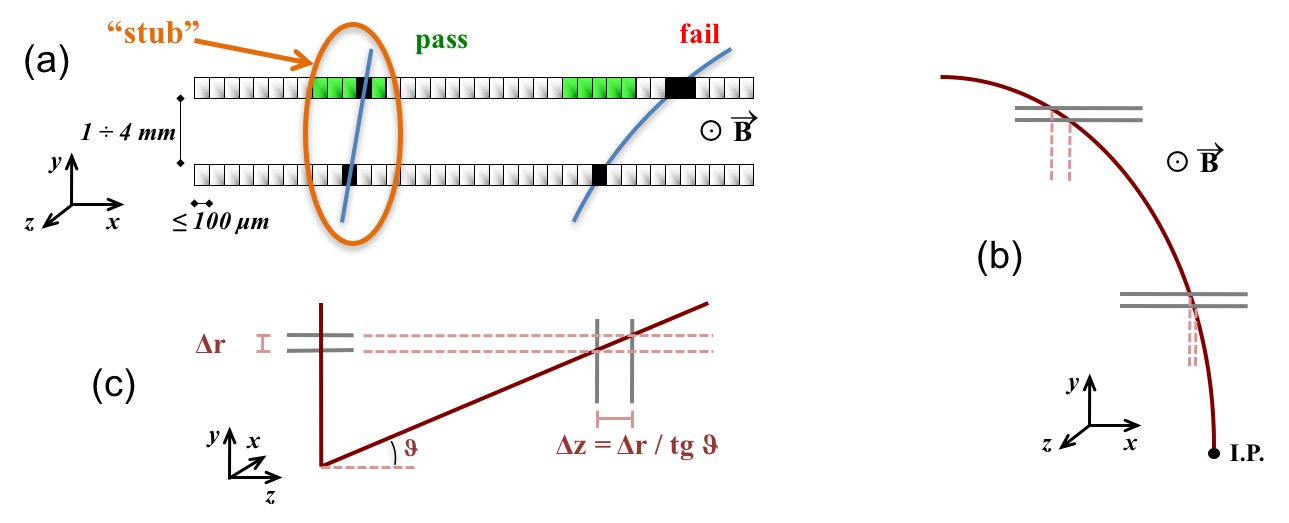
\includegraphics[width=5in]{figs/tk-upgrade/pTsketches.png}
% where an .eps filename suffix will be assumed under latex,
% and a .pdf suffix will be assumed for pdflatex; or what has been declared
% via \DeclareGraphicsExtensions.
\caption{Cluster matching in $p_\mathrm{T}$-modules~\cite{P2TrackerTDR}. (a) Correlating closely spaced clusters between two sensor layers, separated by a few mm, allows discrimination of transverse momentum based on the particle bend in the CMS magnetic field, assuming that the particle originated at the beam-line. (b) The same transverse momentum corresponds to a larger distance between signals for a given sensor spacing. (c) A larger spacing is needed in the endcap disks to achieve the same discrimination. Only tracks with \pT $> 2-3$\GeVc are transferred off-detector.
}
\label{fig:stubs}
\end{figure}

Two \pT modules are being developed for the Outer Tracker upgrade: 2S \emph{strip-strip} modules and PS \emph{pixel-strip} modules, both shown in Fig.~\ref{fig:2Spsmodules}.
The 2S~modules, are designed to be used at radii $r>60$\cm from the beam line, where the hit occupancies are lower and each sensor has an active area of 0.05\cm~$\times$~9.14\cm.
Both 2S~module strip layers have a pitch of 90\mum in the transverse plane, $r$-$\varphi$, and a strip length of 5.03\cm along the direction of the beam axis, $z$.
Each PS~module sensor layer has an active area of 4.69\cm~$\times$~9.60\cm, will be used at radii $20<r<60$\cm where the occupancies are highest.
The upperPS~module layer consist of an upper silicon strip sensor, and the lower a silicon pixel sensor, both with a pitch of 100\mum in $r$-$\varphi$, and a strip length in $z$ of 2.35\cm for the strips and 1.47\mm for the pixels.
The finer granularity provided by the pixel layer affords better resolution along the $z$ axis, which is crucial for vertex identification in the high \PU environment of the HL-LHC.
Further details on the two \pT modules can be found in~\cite{CMS_Upgrade_TP,P2TrackerTDR}.
 
\begin{figure}[tp]
\centering
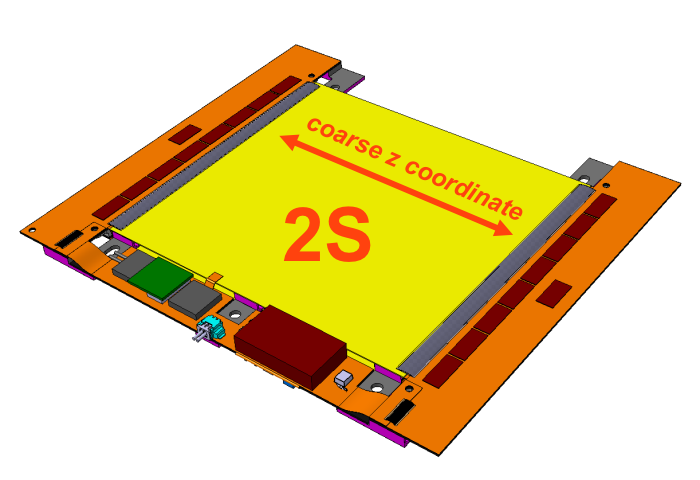
\includegraphics[width=0.55\textwidth,trim={0truecm 0truecm 0truecm 1truecm},clip]{figs/tk-upgrade/2S_assembled.png}
\hfill
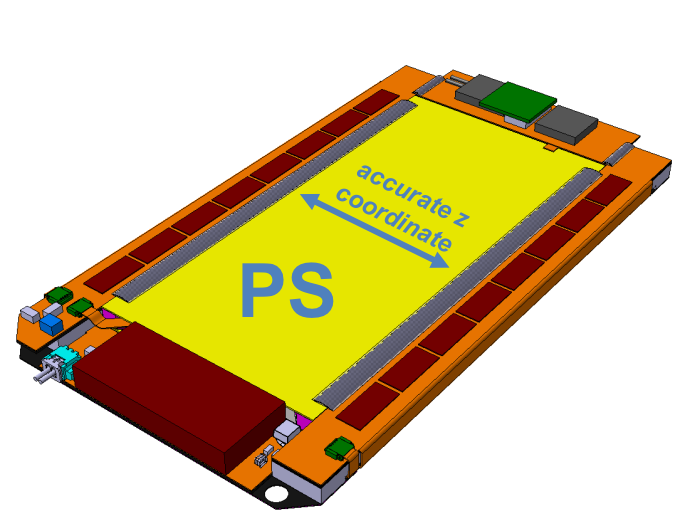
\includegraphics[width=0.44\textwidth,trim={0truecm 0truecm 0truecm 1truecm},clip]{figs/tk-upgrade/PS_assembled.png}
% where an .eps filename suffix will be assumed under latex,
% and a .pdf suffix will be assumed for pdflatex; or what has been declared
% via \DeclareGraphicsExtensions.
\caption{The 2S module (left) and PS module (right), described in the text~\cite{P2TrackerTDR}.}
\label{fig:2Spsmodules}
\end{figure}

The current proposed layout of the Phase-II Outer Tracker, referred to as the \emph{tilted barrel} geometry, is depicted in the upper diagram in Fig.~\ref{fig:trackerlayout}, illustrating the PS and 2S module positions in the six barrel layers and the five endcap disks either side of the barrel.
Only modules located at $|\eta| < 2.4$ will be configured to send stub data off-detector.
The geometry's name is inspired by modules in the three innermost barrel layers being tilted so that their normals point towards the interaction region.
This layout was adopted as it not only improves stub-finding efficiency for tracks with large incident angles but also reduces the overall cost of the system~\cite{P2TrackerTDR}.

\begin{figure}[tbp]
\centering
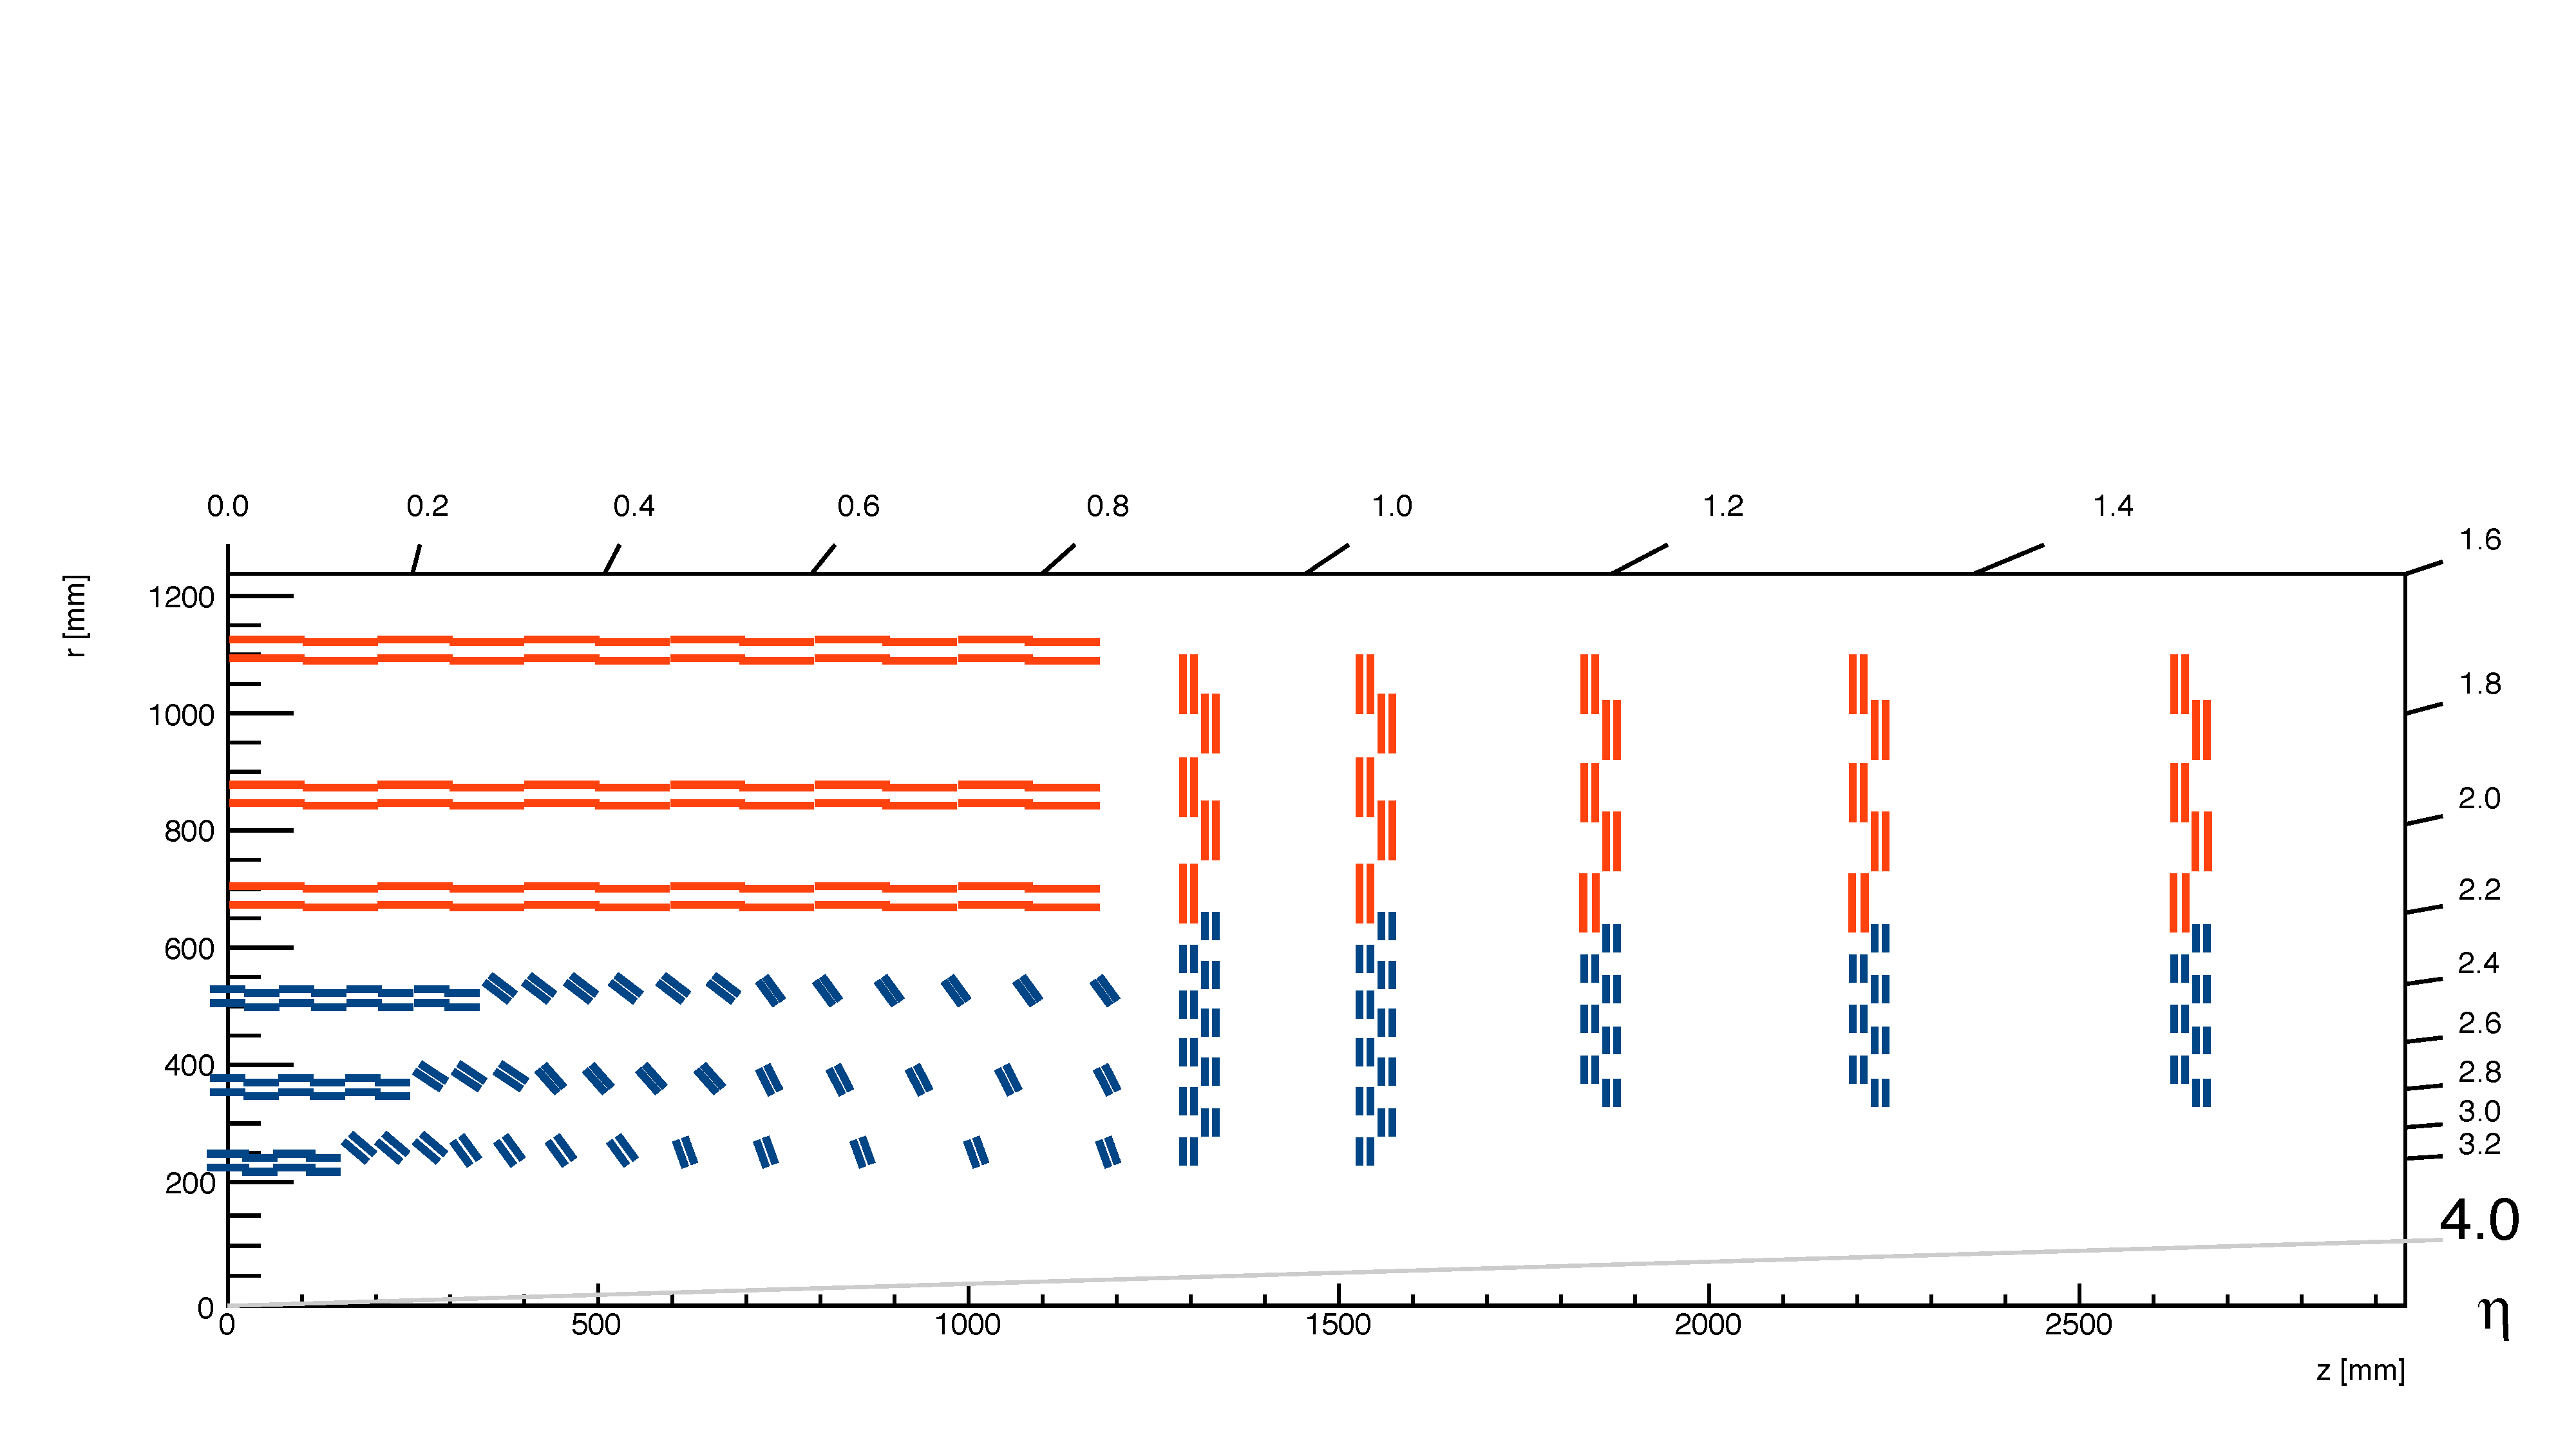
\includegraphics[width=0.8\textwidth,trim={1.1truecm 0truecm 1truecm 12truecm},clip]{figs/tk-upgrade/tiltedbarrelmap.pdf}
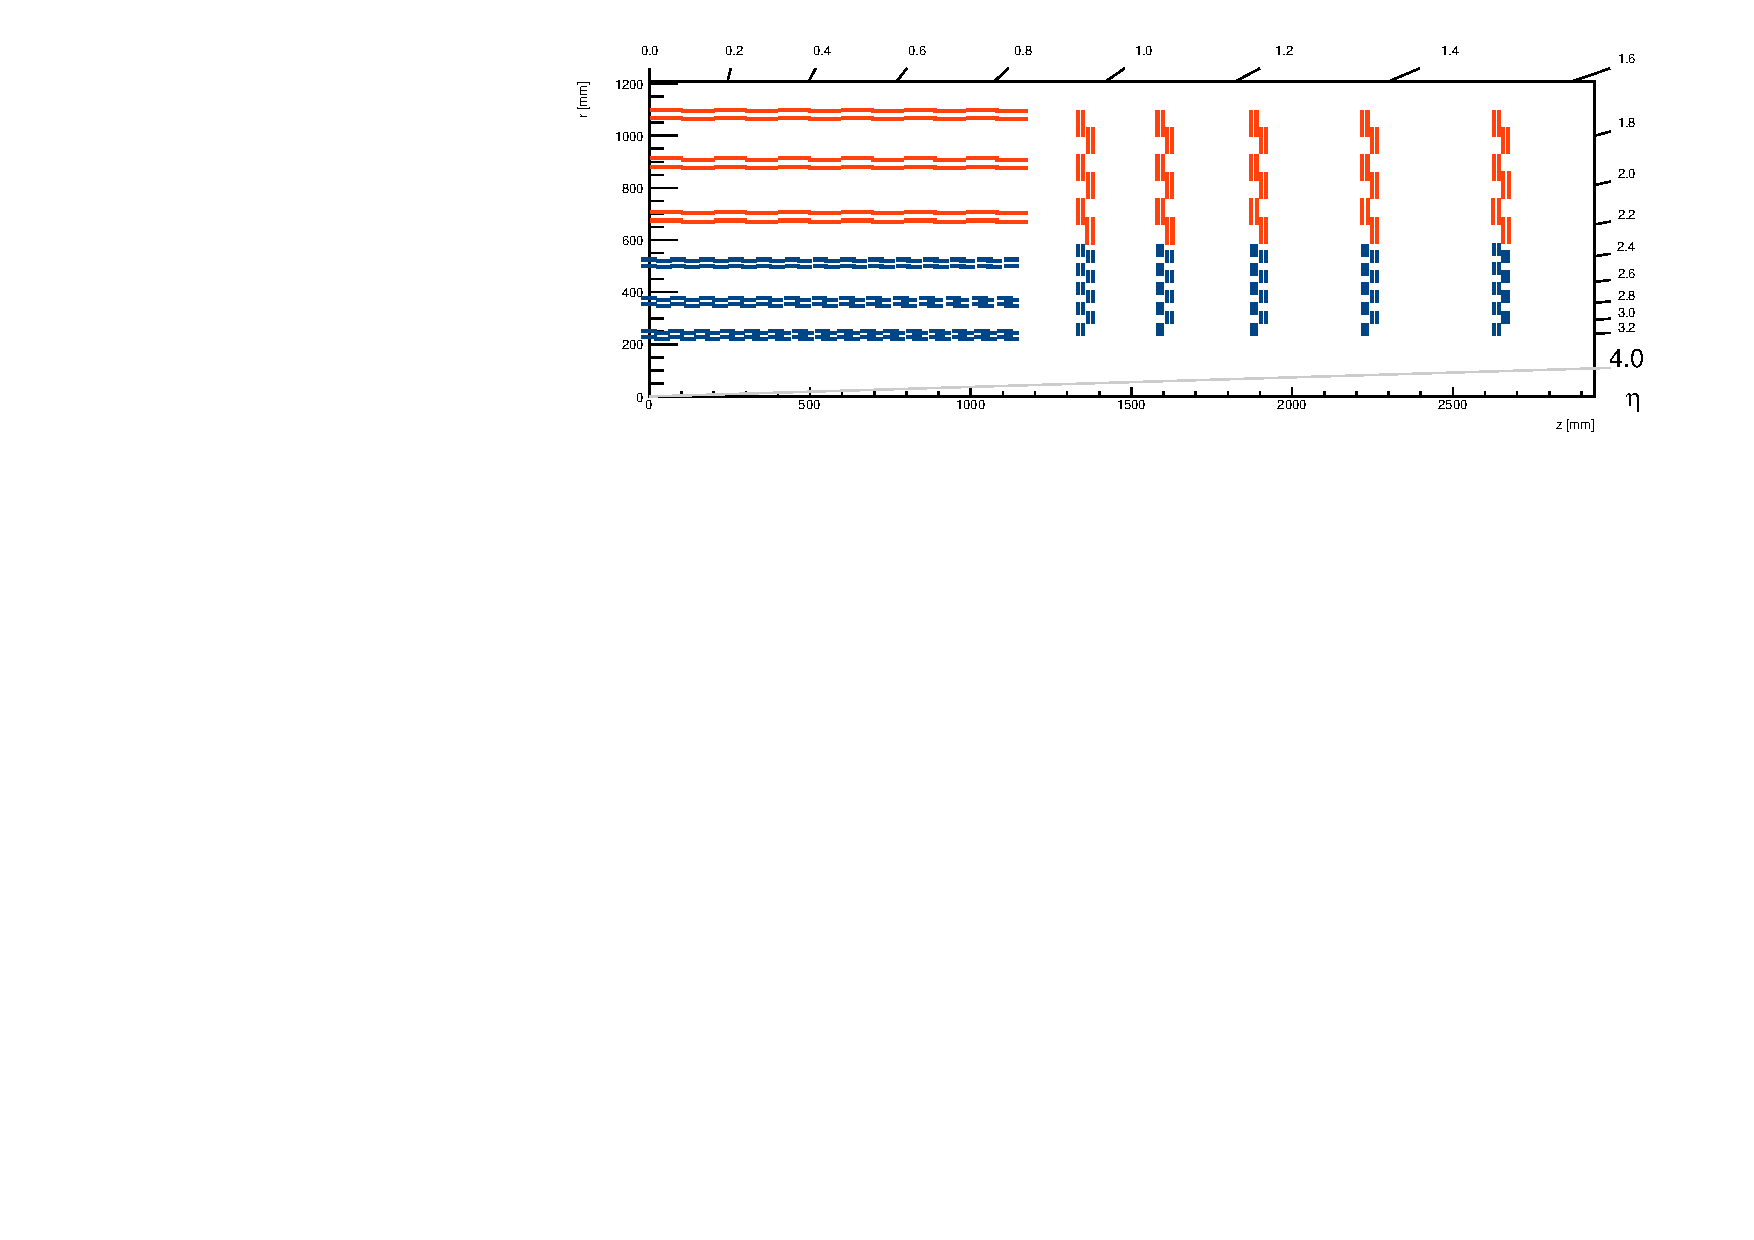
\includegraphics[width=0.8\textwidth,trim={0.7truecm 0truecm 1truecm 0truecm},clip]{figs/tk-upgrade/mersilayout.pdf}
\caption{One quadrant of the Phase-II Outer Tracker layout, showing the placement of the the PS (blue) and 2S (red) modules. The upper diagram shows the currently proposed \emph{tilted barrel} geometry~\cite{tiltedGeometry, P2TrackerTDR}, and the lower diagram shows an older proposal for the layout, known as the \emph{flat barrel} geometry \cite{CMS_Upgrade_TP}.}
\label{fig:trackerlayout}
\end{figure}

Three different L1 track finders, which take the stubs as input and outputs fully reconstructed tracks for the L1, have been explored by the CMS Collaboration.
One uses Associative Memory (``AM'') ASICs for track finding and FPGAs for track fitting, and the other two all-FPGA approaches, one using a Hough Transform (``\HT'') and the other a road search (``tracklet'') algorithm to reconstruct tracks respectively.

Hardware demonstrators for each of the three proposed L1 track finder projects were constructed to prove the feasibility of each approach, which were reviewed in December 2016.
As all of the work discussed in this chapter was on the FPGA-based \HT approach, more detailed descriptions and results of both the AM and tracklet projects' approaches are not discussed here, but are given in~\cite{AM,P2TrackerTDR} and~\cite{tracklet,P2TrackerTDR} respectively.

At the time of the review, the then proposed \emph{flat barrel} geometry~\cite{CMS_Upgrade_TP} was used for all the studies undertaken, as depicted in the lower diagram in Fig.~\ref{fig:trackerlayout}.
Unless stated otherwise, the results discussed below use the old \emph{flat barrel} geometry instead of the currently proposed layout.

\section{An FPGA Based Track Finding Architecture}

Using stubs as an input, the L1 trigger requires input data formatting, track reconstruction and track fitting to be undertaken within an overall latency of 4\mus.  

A scalable, configurable and redundant system architecture based on a fully time-multiplexed design, using current FPGA technology, has been proposed.

A more thorough description of the demonstrator system described is given here~\cite{TMTT_JINST}.

\subsection{Linear $\chi^{2}$ Track Fitter}
A linearised $\chi^{2}$	fit was explored

\subsection{2 GeV Tracking}
The flexibility and robustness

Since the December 2016 demonstrator review, further work on the 